\subsection{Vision}
The image processing algorithm did able to match cards considering all variables, shape, shape count and filler. Results of the image processing can be summarised as follows.
\begin{figure}[position = here]
	\begin{centering}
		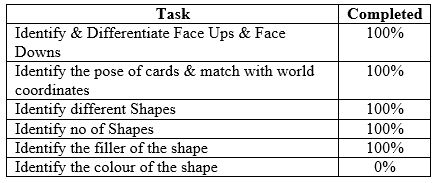
\includegraphics[scale=0.8]{./sachiths_images/image7.png}\\
		\caption[]{\textit{Results Table}}
	\end{centering}
\end{figure}

\textbf{Note:} We only did able to get gray images from the camera as there was a problem with white balancing with the camera driver which we didn't able to fix. If we had rgb images for check the color of the shape we should have check the 3 channels separately and found the dominant channel. 

Results were as following,

1. Shaded one Rectangle
\begin{figure}[position = here]
	\begin{centering}
		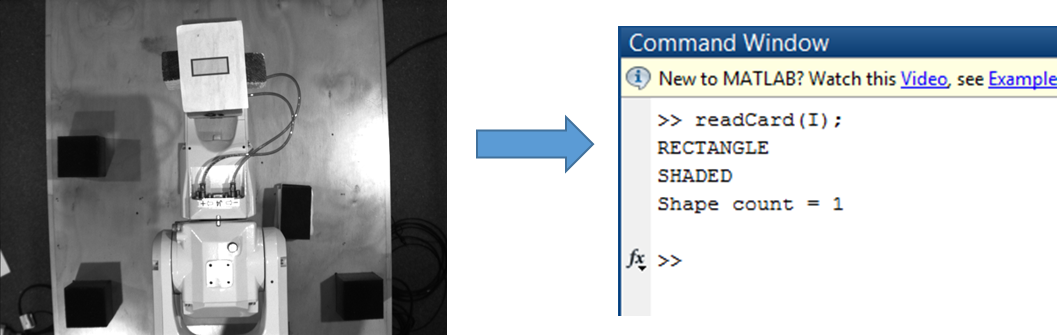
\includegraphics[scale=0.55]{./sachiths_images/image9.png}\\
		\caption[]{\textit{Results for a shaded rectangle}}
	\end{centering}
\end{figure}

2. Block three Rectangles
\begin{figure}[position = here]
	\begin{centering}
		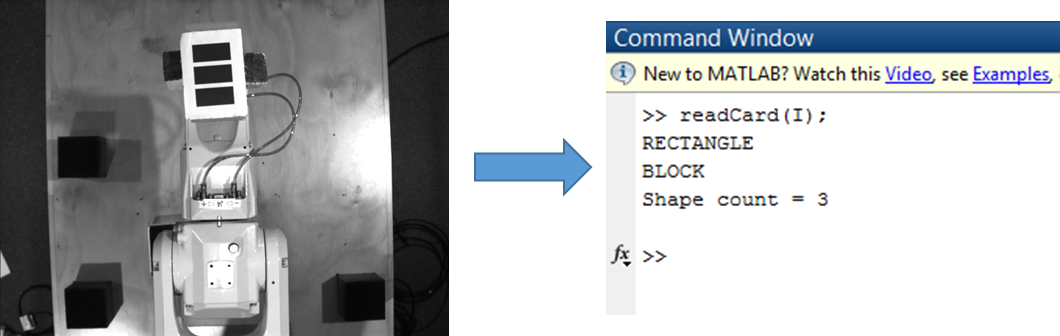
\includegraphics[scale=0.55]{./sachiths_images/image8.png}\\
		\caption[]{\textit{Results for non shaded Triangle}}
	\end{centering}
\end{figure}

3. Shaded one Elipse
\begin{figure}[position = here]
	\begin{centering}
		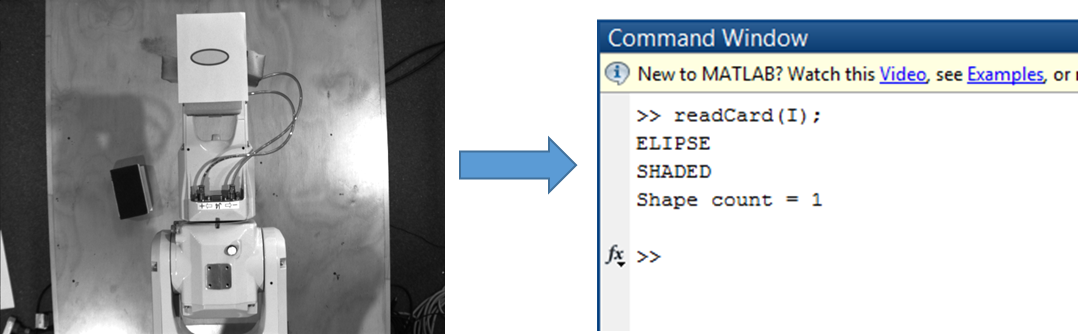
\includegraphics[scale=0.55]{./sachiths_images/image10.png}\\
		\caption[]{\textit{Results for Shaded Elipse}}
	\end{centering}
\end{figure}

